%%%%%%%%%%%%%%%%%%%%%%%%%%%%%%%%%%%%%%%%%%%%%%%%%%%%%%%%%%%%%%%%%%%%%
%%%%%%%%%%%                   PROBLEM 2                   %%%%%%%%%%%
%%%%%%%%%%%%%%%%%%%%%%%%%%%%%%%%%%%%%%%%%%%%%%%%%%%%%%%%%%%%%%%%%%%%%

\section{معرفی سامانه‌ی مکان‌محور مدیریت کارمند (سمک)}

\subsection{هدف استفاده از این سامانه}
این سامانه برای مرتفع کردن نیاز به استخدام نیرو‌های ممیزی و نظارتی به منظور زیر نظر گرفتن روند پیشرفت کار توسط کارمندان ایجاد و ارائه خواهد شد.

مدیران کسب‌وکار‌ها به وسیله‌ی این سامانه خواهند توانست فرایند سرکشی و نظارت لحظه‌ای به کار کارمندان، تخصیص کار به آنها و گزارش‌گیری از روند انجام کار را به صورت خودکار انجام دهند.

همچنین این سامانه قادر خواهد بود نیاز‌هایی همچون مدیریت درآمد‌ها و مخارج کارمندان و سیستم را بر عهده گرفته و مرتفع کند.

\subsection{نوع در‌آمد}
درآمد اصلی این سامانه با فروش اشتراک استفاده از آن بسته به نیاز‌ کاربران و مدیران و در بسته‌های قیمتی متفاوت خواهد بود. به صورت خلاصه، به ازای هر شرکت-کارمند-ماه تحت پوشش سامانه، هزینه‌ی اشتراک از مدیریت آن شرکت اخذ خواهد شد.

\subsection{تعداد افراد درگیر}
ذی‌نفعان مورد انتظار این سامانه در زمان نگارش این مستند عبارتند از:

\begin{itemize}
\item 
مدیریت کسب و کار‌هایی که کارمندان در آنها دائما دور از مدیریت و در تردد هستند .
\item
افرادی که توسط مدیریت مورد نظارت خواهند بود. اعم از بازاریابان یا مسئولین فروش یا کارمندان.
\item
افرادی که مدیریت، نگهداری و پشتیبانی سامانه را بر عهده خواهند داشت.
\end{itemize}

همچنین به نظر می‌رسد برای توسعه‌ی چنین سیستمی بهره‌گیری از تیمی خبره و حداکثر ۱۰ نفره مناسب خواهد بود.

\subsection{میزان موفقیت، سیستم‌عامل، زبان برنامه نویسی، متن باز بودن، ...}
این سامانه هنوز تولید نشده بنابر‌این نمی‌توان در مورد میزان موفقیت آن اظهار نظر کرد.

همچنین در گام تحلیل بایستی از هرگونه درگیری در جزئیات قلمرو پاسخ  خودداری شود بنابراین وضع سیستم در حوزه‌هایی مانند سیستم‌عامل، زبان برنامه نویسی و متن باز بودن مشخص نیست.


\subsection{معرفی قابلیت‌های اصلی}

\begin{enumerate}
\item کاربران میهمان باید بتوانند در سیستم ثبت نام کنند.
\item کاربران ثبت نام کرده باید بتوانند نسبت به خرید یکی از بسته‌های پیشنهادی برای مدیریت کسب و کار خود اقدام کنند. در این صورت سطح دسترسی مدیریت آن کسب و کار را دریافت خواهند کرد.
\item کاربران مدیر باید بتوانند کاربران دیگر را به عنوان کارمند به کسب و کار خود دعوت کنند. کاربر مورد نظر می‌تواند دعوت را تایید یا آن را رد کند.
\item کاربران باید بتوانند نسبت به ویرایش اطلاعات کاربری خود اقدام کنند.
\item کاربران مدیر باید بتوانند نسبت به ویرایش اطلاعات کسب و کار خود اقدام کنند.
\item کاربران مدیر باید بتوانند اطلاعات حقوقی کارمندان خود را ویرایش کرده یا کارمند را حذف کنند.
\item کاربران باید بتوانند با وارد کردن نام کاربری و کلمه‌ی عبور خود وارد پنل کاربری‌شان شوند.
\item کاربران باید بتوانند با درخواست خروج از سامانه خارج شوند.
\item کاربران باید بتوانند درخواست فراموشی رمز عبور را صادر و فرایند بازیابی رمز را شروع کنند.
\item مدیر کل سامانه باید بتواند اعلانات سامانه را مدیریت کرده و در صورت لزوم اعلان جدید اضافه کند و یا اعلان‌های قبلی را ویرایش یا حذف کند.
\item مدیر کل سامانه باید بتواند به صورت دستی از اطلاعات سامانه پشتیبانی تهیه کند.
\item پشتیبانی خودکار اطلاعات باید در بازه‌های زمانی منظم توسط سامانه انجام شود.
\item مدیران کسب و کار باید بتوانند نسبت به ثبت ردیاب برای کارمندان  خود اقدام کنند.
\item مدیران کسب و کار باید بتوانند نسبت به ویرایش یا حذف ردیاب کارمندان  خود اقدام کنند.
\item مدیران کسب و کار باید بتوانند شیفت‌های کاری خاص را به کارمندان خود تخصیص داده یا شیفت کاری کارمند را ویرایش کنند.
\item مدیران کسب و کار باید بتوانند در هر لحظه موقعیت مکانی کارمندان خود را ردیابی کنند.
\item موقعیت مکانی کارمندان باید در بازه‌های زمانی منظم ثبت شود.
\item مدیران کسب و کار باید بتوانند گزارش مسیر‌های روزانه‌ی کارمند را مشاهده کنند.
\item مدیران کسب و کار باید بتوانند گزارش فعالیت‌های روزانه‌ی کارمندان خود را مشاهده کنند.
\item سامانه باید هر روز کاری نسبت به انجام حضور و غیاب کارمندان در وقت از پیش تعیین شده توسط مدیر کسب و کار اقدام کند.
\item مدیران کسب و کار باید بتوانند گزارش دوره‌ای هزینه‌های پنل را دریافت کنند.
\item مدیران کسب و کار باید بتوانند گزارش دوره‌ای درآمد‌های پنل را دریافت کنند.
\item مدیران کسب و کار باید بتوانند گزارش دوره‌ای فعالیت‌های انجام شده را دریافت کنند.
\item مدیران کسب و کار باید بتوانند از طریق سامانه، دستمزد کارمندان خود را به صورت خودکار محاسبه کنند.
\item مدیران کسب و کار باید بتوانند گزارش دوره‌ای سفارشات ثبت شده در پنل را دریافت کنند.
\item مدیران کسب و کار باید بتوانند در هر لحظه گزارش وظایف انجام شده و ساعات مفید کاری هر کارمند را مشاهده کنند.
\item مدیران کسب و کار باید بتوانند نسبت به دریافت و ثبت سفارش جدید با مشخص کردن موقعیت مکانی، در سامانه اقدام کنند.
\item مدیران کسب و کار باید بتوانند جزئیات سفارش ثبت شده را ویرایش و یا آن را حذف کنند.
\item مدیران کسب و کار باید بتوانند در هر لحظه وضعیت انجام سفارش توسط کارمندان را پیگیری کنند.
\item مدیران کسب و کار باید باید بتوانند در هر لحظه یک سفارش را به  مناسب ترین کارمند (نزدیک ترین جغرافیایی یا در دسترس ترین) الصاق کنند.
\item کارمندان باید بتوانند در هر لحظه وضعیت انجام سفارش در سامانه را به روز رسانی کنند. همچنین امکان به روز رسانی خودکار وضعیت سفارش بر اساس موقعیت مکانی کارمند بایستی وجود داشته باشد.
\item کارمندان باید بتوانند از طریق سامانه از مدیریت کسب و کار تقاضای مرخصی کنند.
\item کارمندان باید بتوانند از طریق سامانه از مدیریت کسب و کار تقاضای تخصیص شیفت شناور بدهند.
\item کارمندان باید بتوانند از طریق سامانه به مدیریت کسب و کار پیام ارسال کنند.
\item مدیران کسب و کار باید بتوانند به یک کارمند خاص پیام ارسال کنند.
\item مدیران کسب و کار باید بتوانند برای تمامی کارمندان اعلان عمومی ارسال کنند.
\item سامانه باید برای مسیر‌های طی شده توسط کارمندان، تخمین زمانی مناسبی را محاسبه کرده و با زمان انجام کار توسط کارمند مقایسه کند.
\end{enumerate}

\subsection{نمودار موارد کاربری}


\subsubsection{زیرسیستم‌ها}
سیستم نرم‌افزاری ما از ۶ زیرسیستم مجزا تشکیل شده است که عبارتند از:

\begin{enumerate}
\item زیرسیستم ثبت نام و ورود
\item زیرسیستم مدیریت کارمندان
\item زیرسیستم مدیریت سفارشات و مشتریان
\item زیرسیستم مدیریت مالی و گزارشات
\item زیرسیستم پیام‌رسانی و اعلانات
\item زیرسیستم مدیریت سامانه
\end{enumerate}


%%%%%%%%%%%%%%%%%%%%%%%%%%%%%%%%%%%%%%%%%%%%%%%%%%%%%%%%%%%%%%%%
\subsubsection{راهنمای نمودار}
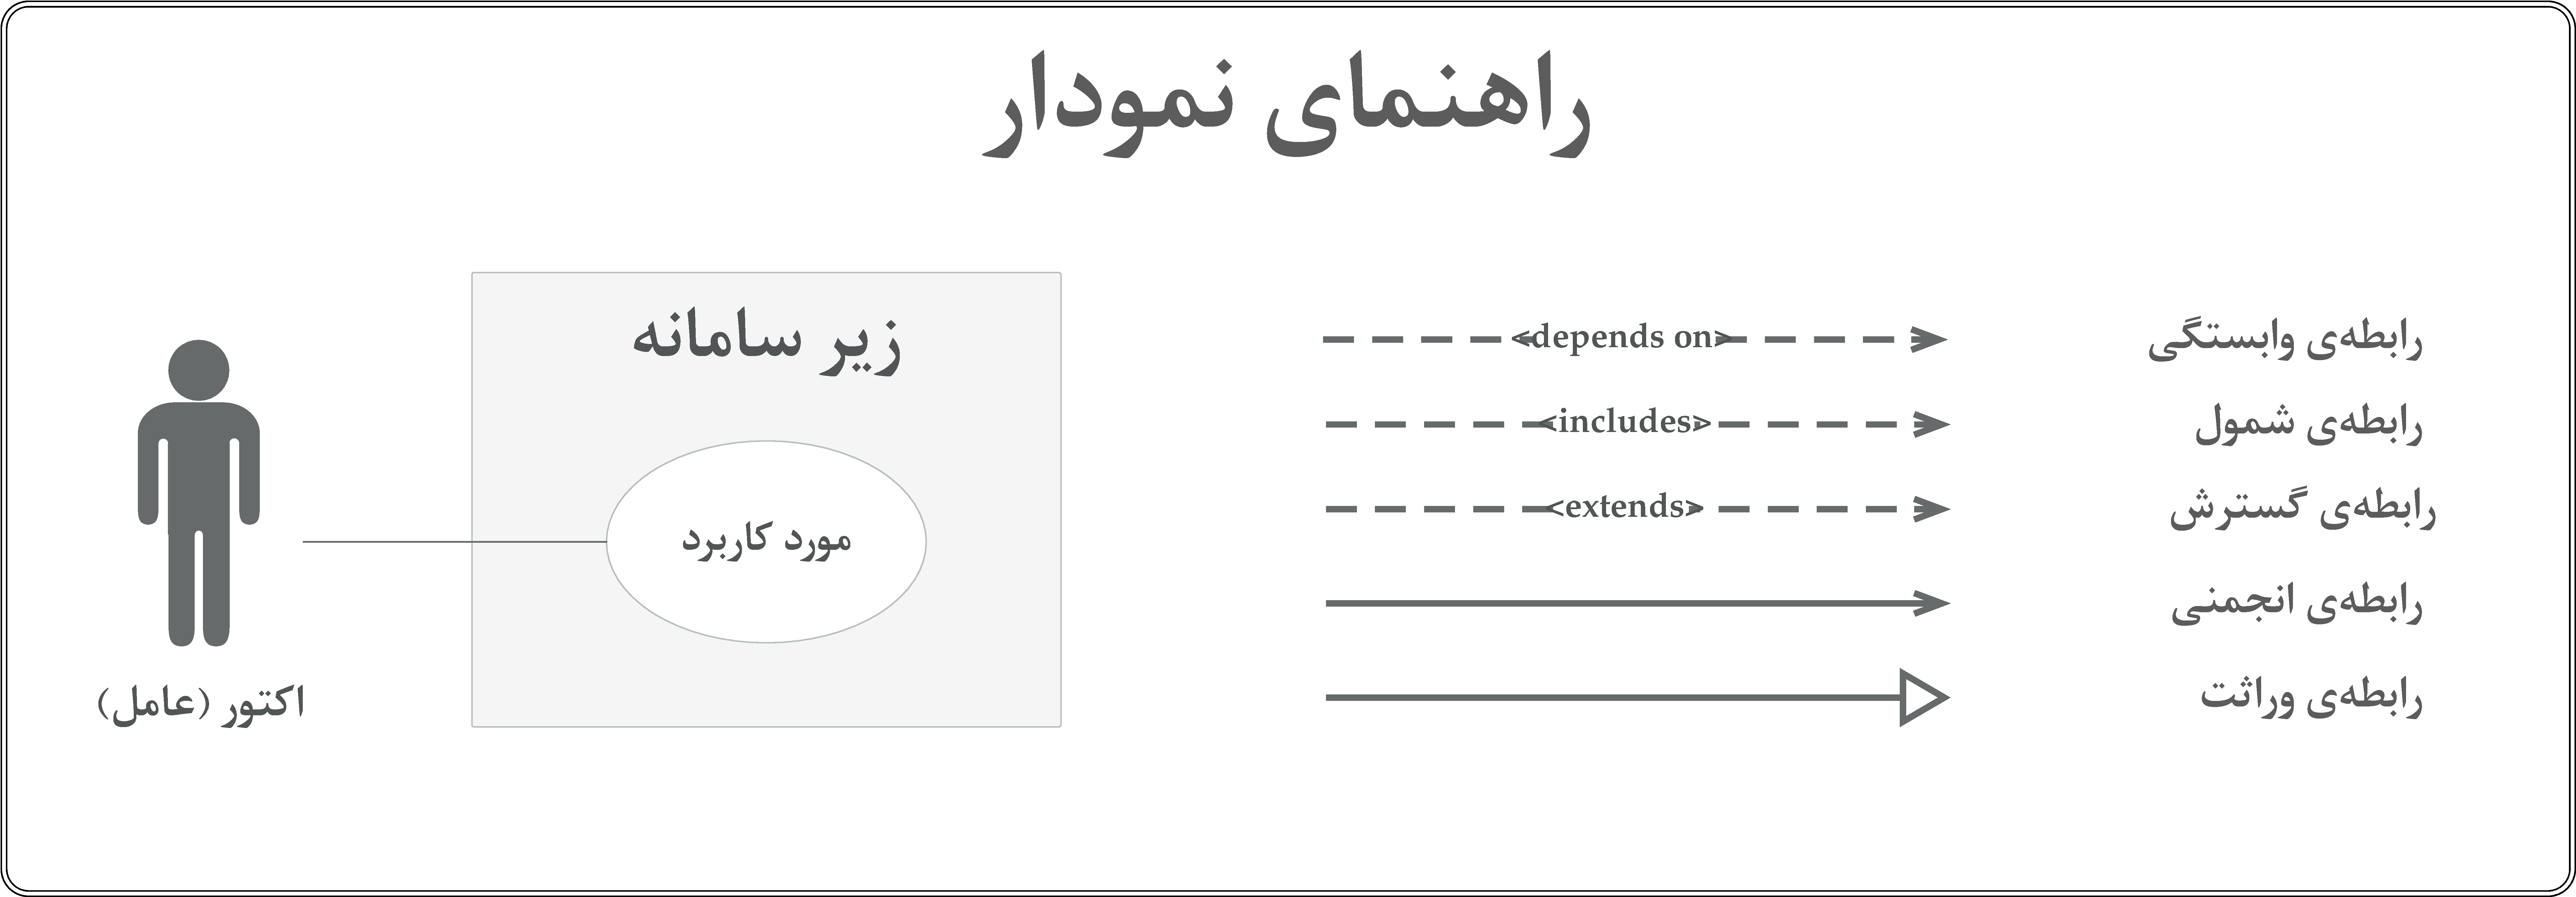
\includegraphics[width = \textwidth]{images/legend}
%%%%%%%%%%%%%%%%%%%%%%%%%%%%%%%%%%%%%%%%%%%%%%%%%%%%%%%%%%%%%%%%
\subsubsection{کاربران سامانه}
کاربران سامانه‌ی سمک عبارتند از:
\begin{enumerate}
\item مدیران کسب‌وکار
\item کارمندان آنها
\item مدیریت و پشتیبانی سامانه‌ی سمک
\end{enumerate}

برای ترسیم نمودار  سامانه وجود این کنش‌گر‌ها مورد تصور است:
\begin{center}
\begin{tabular}{|c|c|}
\hline
\rowcolor{black!30}
کنش‌گر
&
توضیحات
\\ \hline
مدیر کل سامانه
&
فرد یا افراد مسئول نگهداری، پشتیبانی و توسعه‌ی سیستم
 \\ \hline

زمان
&
کنش‌گر مرتبط با انجام کار‌هایی که به صورت دوره‌ای یا در زمانی خاص انجام می‌شوند.
 \\ \hline
بانک
&
درگاه پرداخت بانکی مورد استفاده برای انجام تراکنش‌ها
 \\ \hline
حسگر مکان
&
قطعه‌ای سخت افزاری که موقعیت جغرافیایی خود را به سیستم گزارش می‌دهد.
 \\ \hline
کارمند
&
یک فرد حقوقی که برای یک مدیر کسب و کار فعالیت کرده و پاداش دریافت می‌کند
 \\ \hline
مدیر کسب‌وکار
&
فردی حقوقی که مسئولیت مدیریت و اداره‌ی یک کسب‌و‌کار را بر عهده دارد.
 \\ \hline
کاربر ثبت شده
&
هر یک از کاربران سامانه که در آن تشکیل حساب کاربری داده باشند.
 \\ \hline
کاربر میهمان
&
هر یک از کاربران سامانه که هنوز در آن تشکیل حساب نداده باشند.
 \\ \hline
کاربر سامانه
&
به تمامی کاربران سامانه اطلاق می‌شود.
 \\ \hline
	
\end{tabular}
\end{center}
\includegraphics[width = \textwidth]{images/actors}
%%%%%%%%%%%%%%%%%%%%%%%%%%%%%%%%%%%%%%%%%%%%%%%%%%%%%%%%%%%%%%%%
\subsubsection{زیرسیستم ثبت نام و ورود}
\includegraphics[width = \textwidth]{images/registration-man}
%%%%%%%%%%%%%%%%%%%%%%%%%%%%%%%%%%%%%%%%%%%%%%%%%%%%%%%%%%%%%%%%
\subsubsection{زیرسیستم مدیریت کارمندان}
\includegraphics[width = \textwidth]{images/employee-man}
%%%%%%%%%%%%%%%%%%%%%%%%%%%%%%%%%%%%%%%%%%%%%%%%%%%%%%%%%%%%%%%%
\subsubsection{زیرسیستم مدیریت سفارشات و مشتریان}
\includegraphics[width = \textwidth]{images/order-customer-man}
%%%%%%%%%%%%%%%%%%%%%%%%%%%%%%%%%%%%%%%%%%%%%%%%%%%%%%%%%%%%%%%%
\subsubsection{زیرسیستم مدیریت مالی و گزارشات}
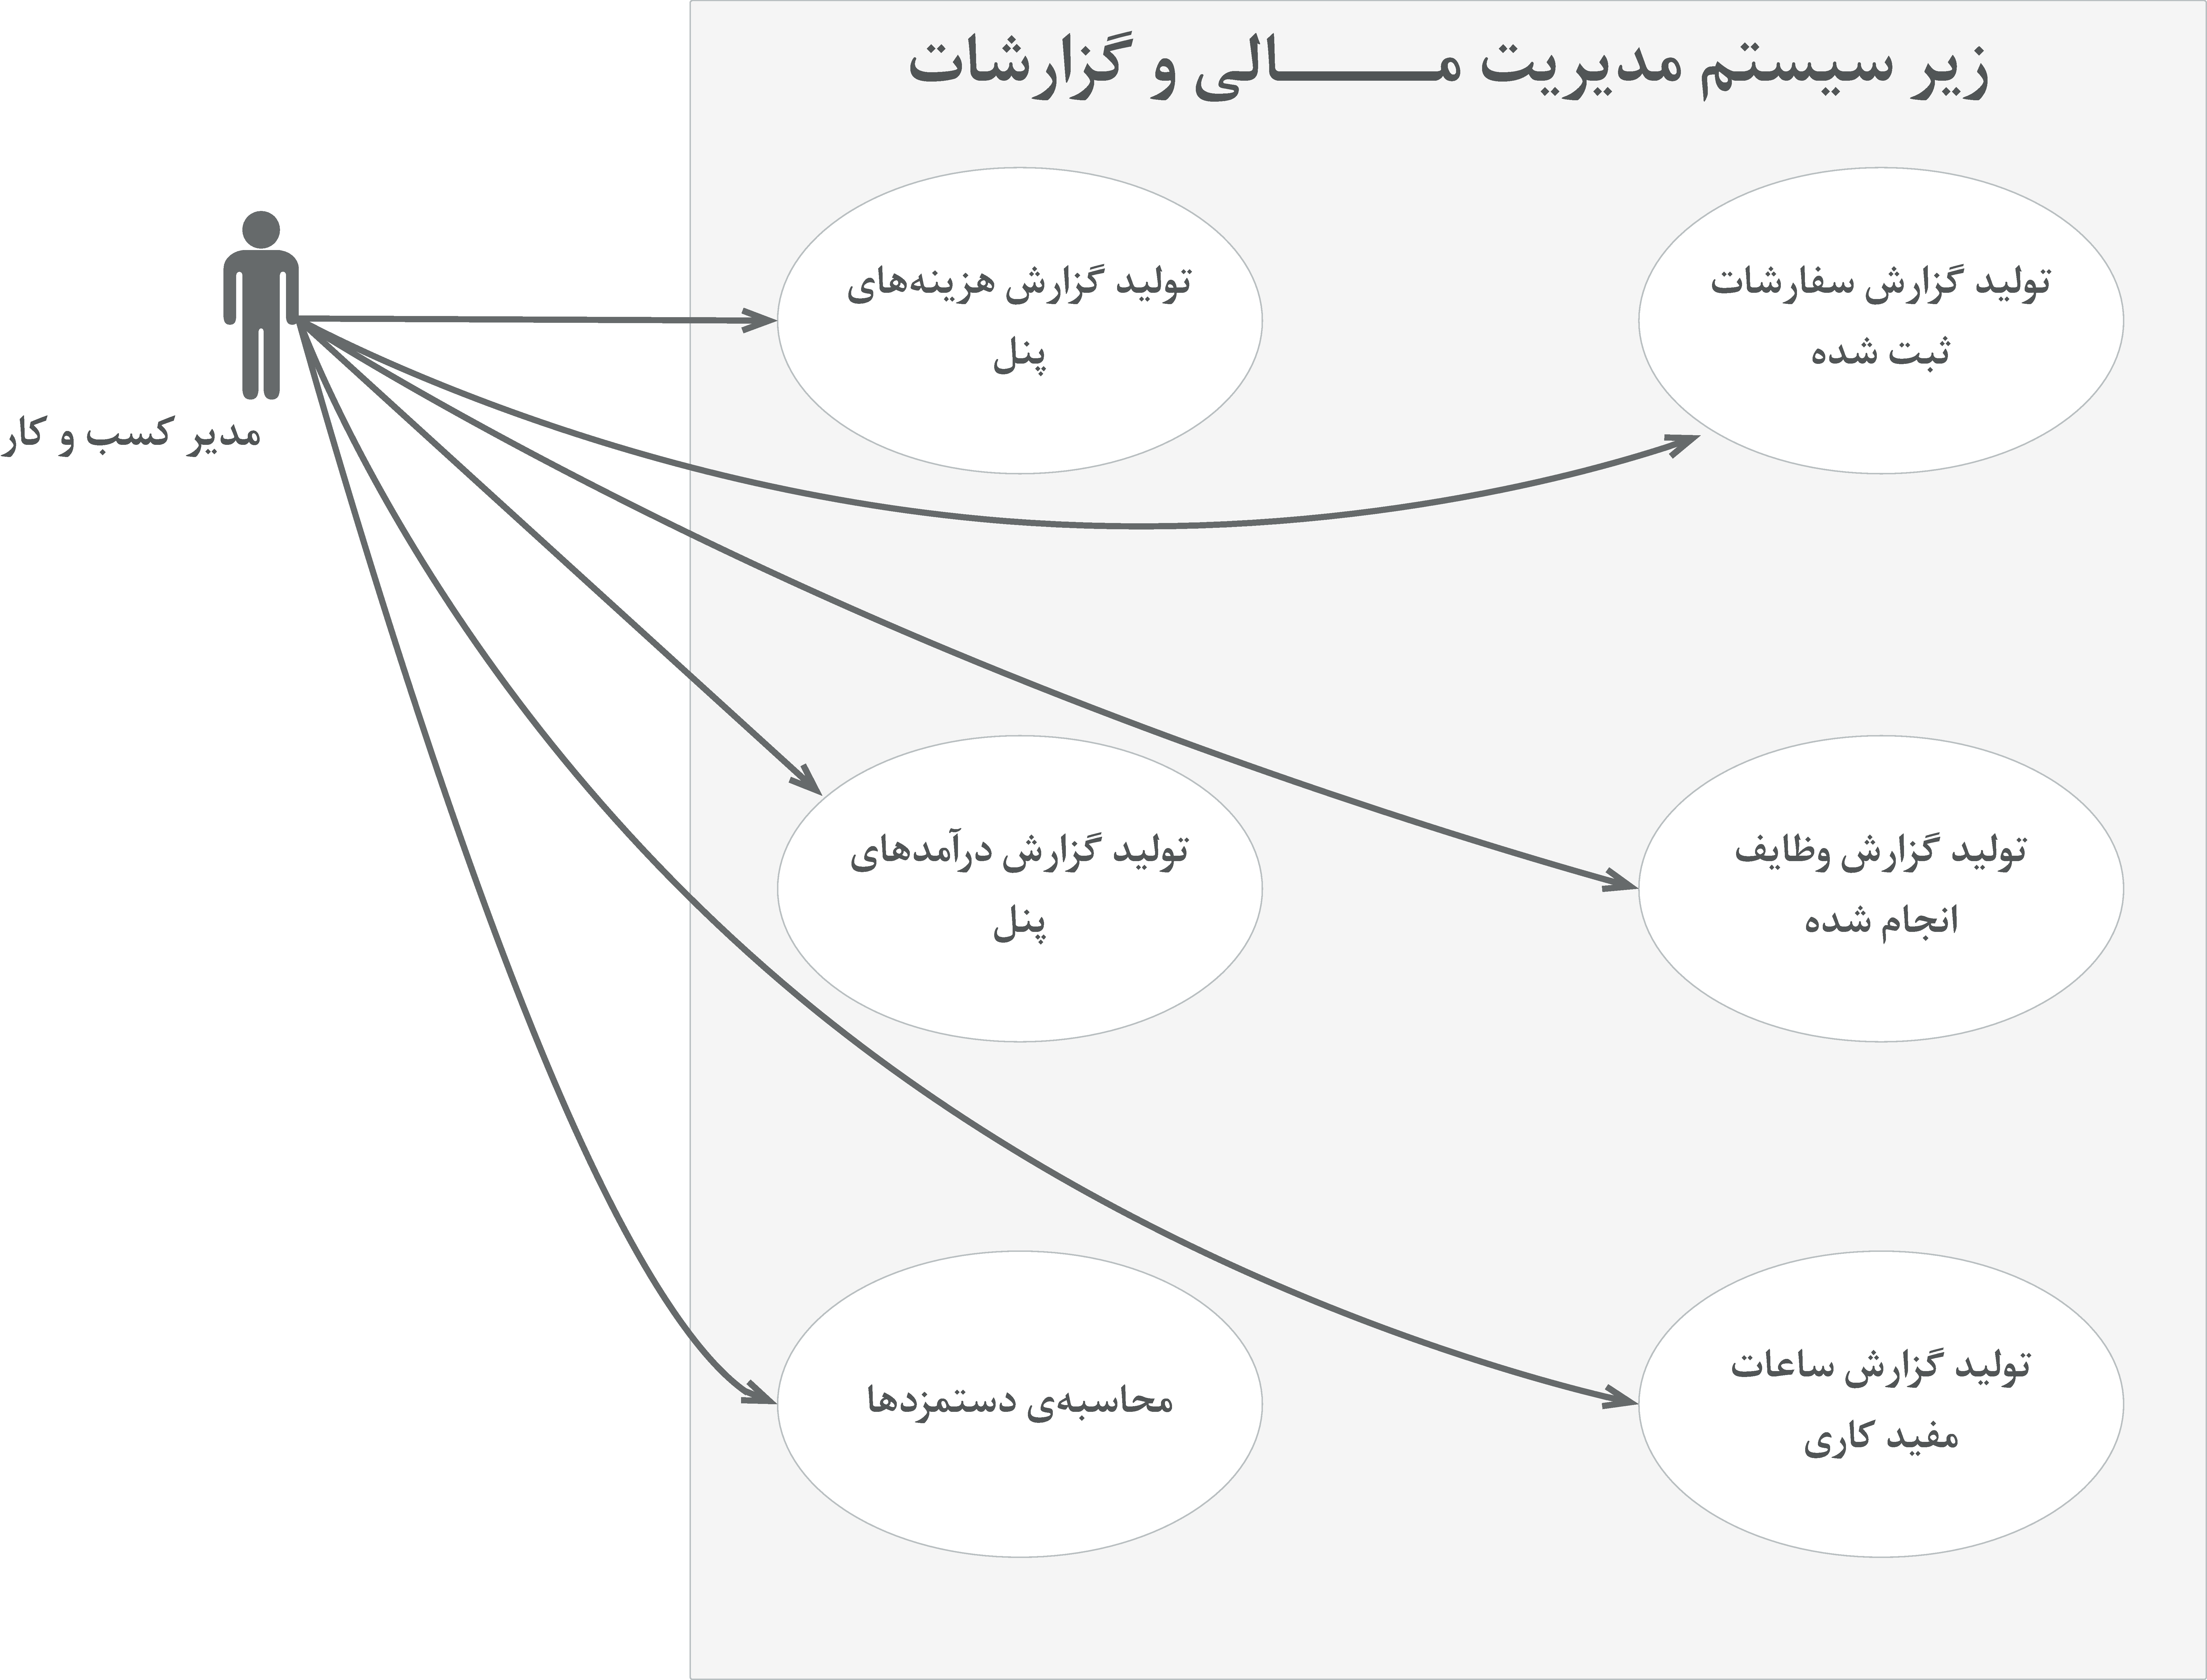
\includegraphics[width = \textwidth]{images/financial-man}
%%%%%%%%%%%%%%%%%%%%%%%%%%%%%%%%%%%%%%%%%%%%%%%%%%%%%%%%%%%%%%%%
\subsubsection{زیرسیستم پیام‌رسانی و اعلانات}
\includegraphics[width = \textwidth]{images/messaging-man}
%%%%%%%%%%%%%%%%%%%%%%%%%%%%%%%%%%%%%%%%%%%%%%%%%%%%%%%%%%%%%%%%
\subsubsection{زیرسیستم مدیریت سامانه}
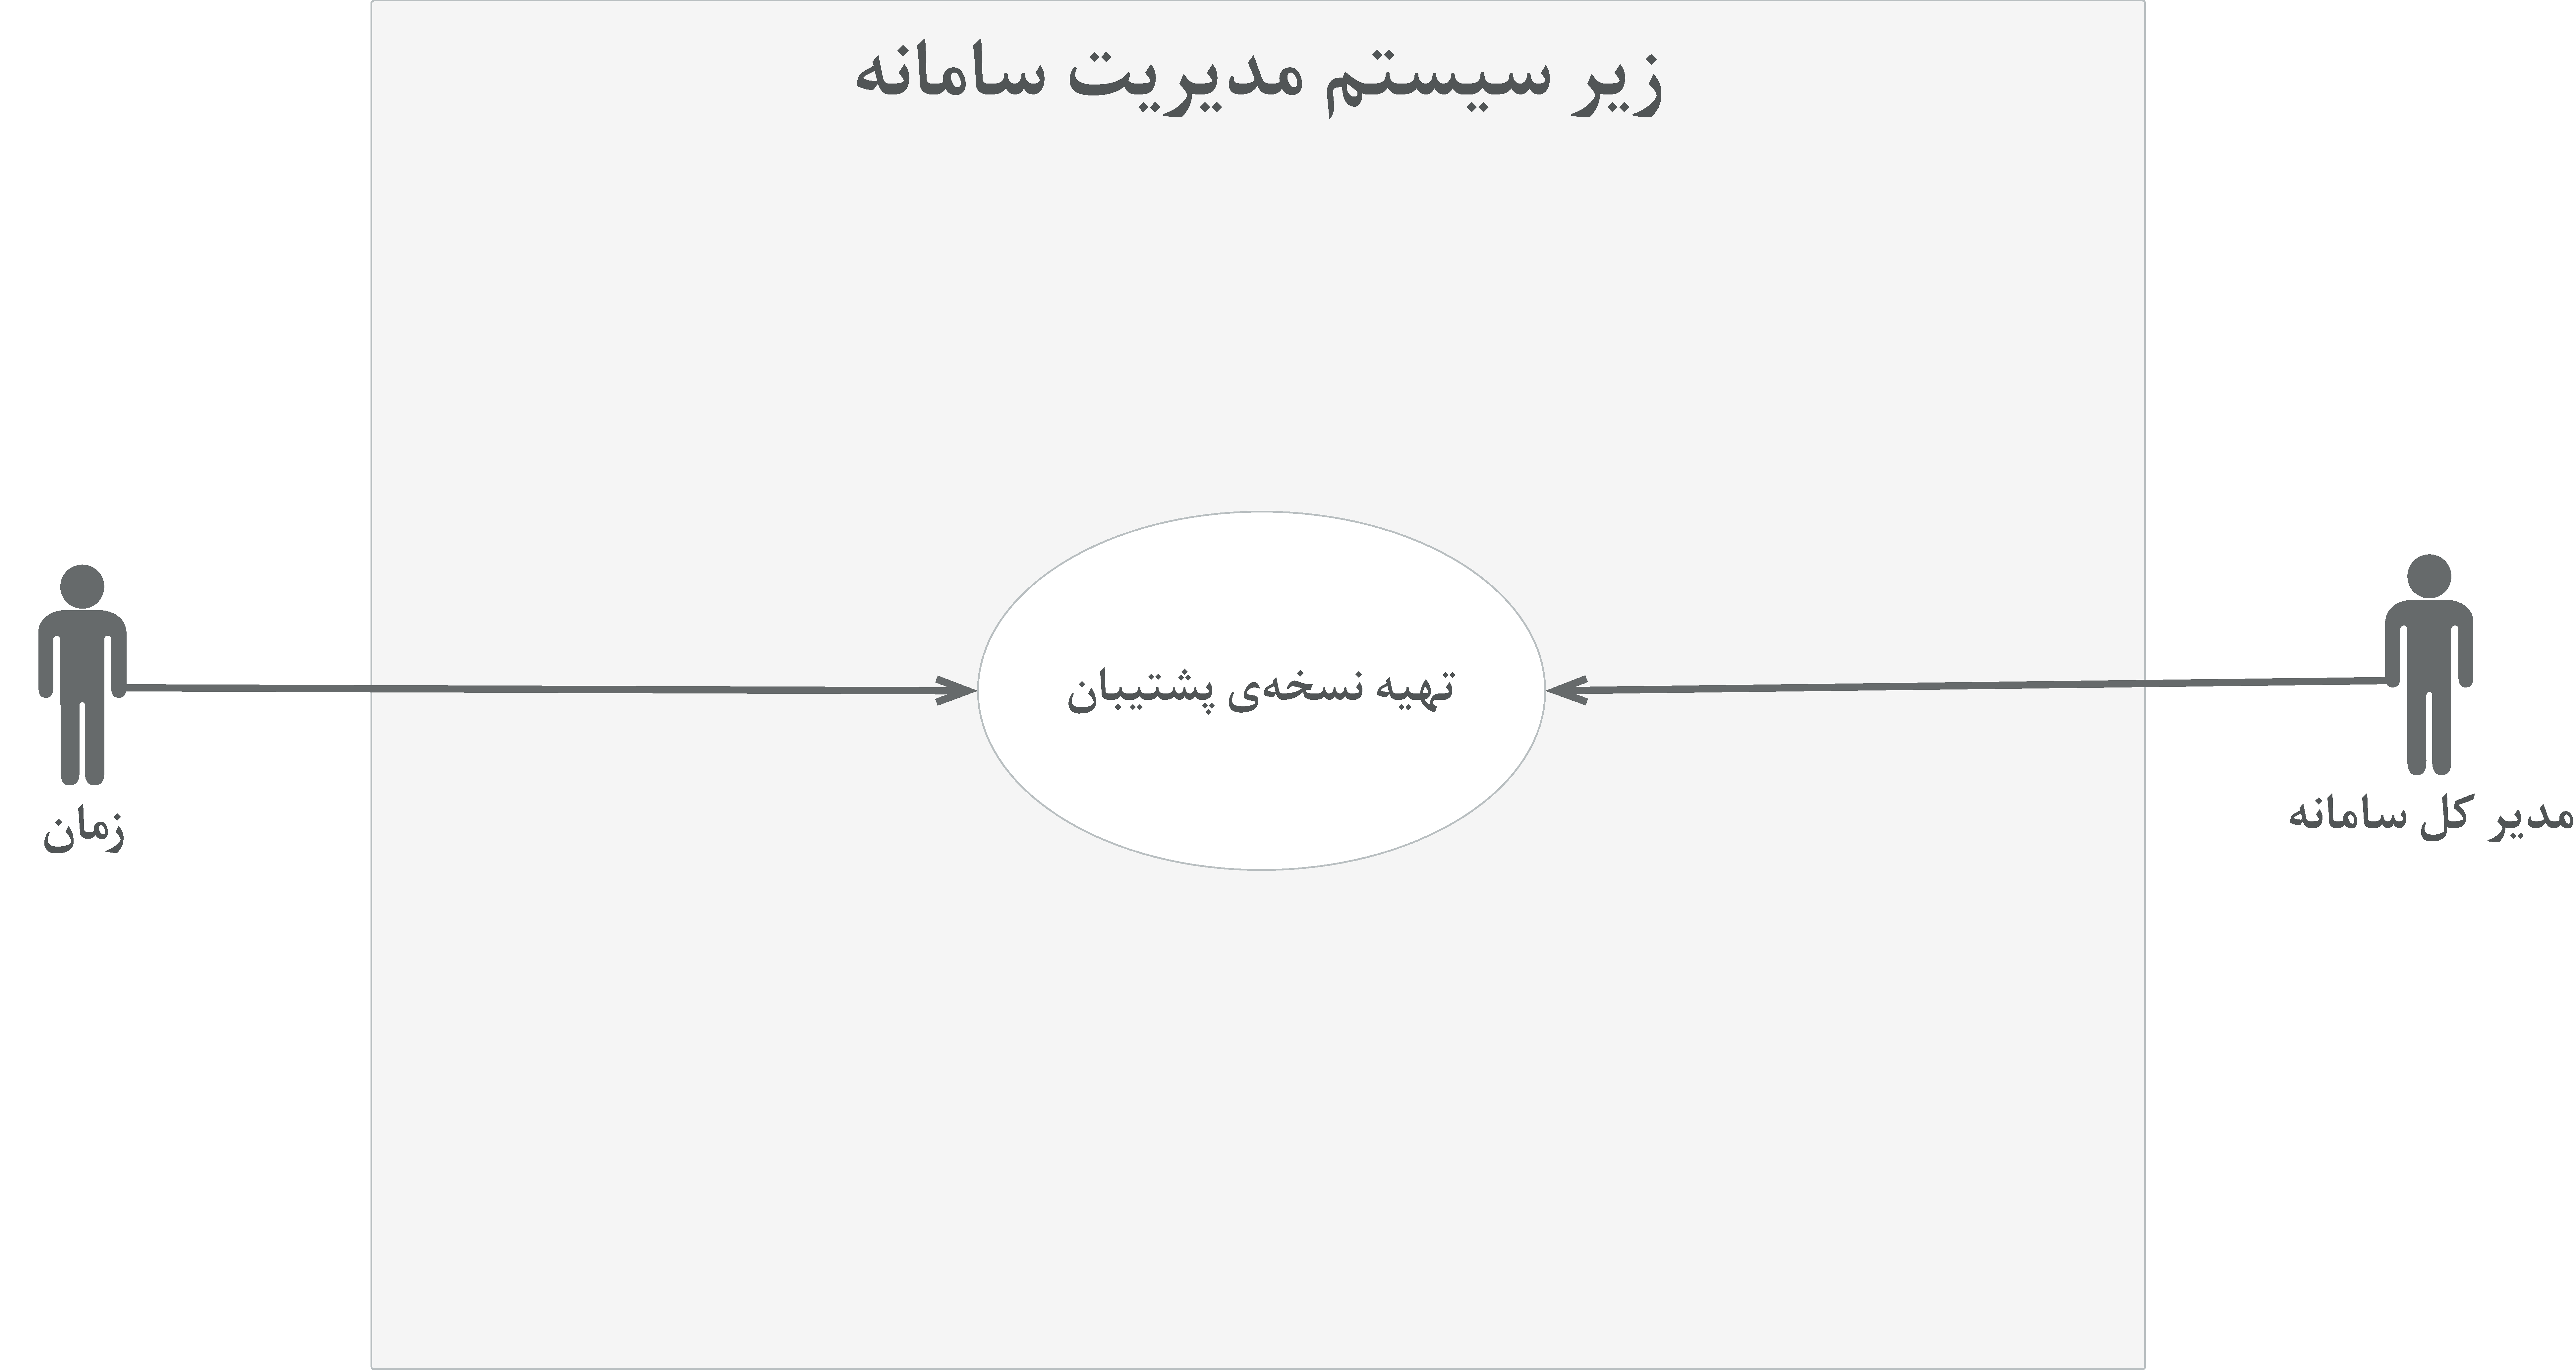
\includegraphics[width = \textwidth]{images/system-man}


\subsection{نکات قوت سامانه‌ی جدید نسبت به موارد بررسی شده}
سامانه‌ی جدید نسبت به موارد بررسی شده در قبل دارای برتری‌هایی است که از میان آنها می‌توان به این موارد اشاره کرد:


\begin{itemize}
\item 
مفهوم ردیاب در این سامانه به صورت کلی در نظر گرفته شده است و می‌توان در آن از هرگونه دستگاهی که مجهز به اینترنت و ماژول موقعیت‌سنج باشد به عنوان ردیاب استفاده کرد.

به این صورت کارمندان و مدیران کسب‌وکار بسته به ترجیحشان می‌توانند از وسیله‌ی مناسب استفاده کنند.

\item
سیستم قابلیت تعیین معیاری برای تخصیص بهترین کارمند به یک سفارش را در اختیار قرار می‌دهد. به این صورت می‌توان بر اساس اولویت موضوع، کارمند خبره‌تر، نزدیک‌تر یا با وظایف فعلی کمتر را برای انجام کار تعیین کرد.

\item
سیستم سعی می‌کند برای مدت زمان انجام سفارش تخمینی مناسب را محاسبه کند. از حاصل این تخمین و رضایت مشتری می‌توان معیاری مناسب برای صحت عملکرد کارمند استخراج کرد.

\item
سیستم امکان به روز رسانی خودکار یا دستی را برای انجام سفارش به کارمندان  می‌دهد. به این صورت میزان پیشرفت سفارش با توجه به موقعیت مکانی کارمند برآورد شده و مقدار قابل ملاحظه‌ای  در زمان مفید کاری صرفه‌جویی می‌شود.

\item 
این سیستم بر خلاف دو سیستم قبل سعی کرده تمامی روابط بین کارمندان و مدیریت کسب و کار را مورد پوشش خود قرار دهد. به این صورت انجام دورکاری و مدیریت از فاصله‌های دور نیز میسر خواهد شد.

\end{itemize}